\documentclass[a4paper,fleqn,usenatbib]{mnras}
%\usepackage{newtxtext,newtxmath}
\usepackage[T1]{fontenc}
\usepackage{ae,aecompl}
\usepackage{graphicx}	% Including figure files
\usepackage{amsmath}	% Advanced maths commands
\usepackage{amssymb}	% Extra maths symbols
\usepackage{epstopdf}
\usepackage{hyperref}
\usepackage{tikz}
%\usepackage{pgflots}

\def\grs{{GRS\,1739--278\,}}
\def\swiftx{{\em Swift-XRT\,}}
\def\swiftb{{\em Swift-BAT\,}}
\def\xmm{{\em XMM-Newton\,}}
\def\nustar{{\em NuSTAR\,}}
\def\integral{{\em INTEGRAL\,}}
\def\maxi{{\em MAXI\,}}


\def\ferg{erg~cm$^{-2}$~s$^{-1}$}
\def\arcsec{''}
\def\degr{$^\circ$}
\def\arcmin{'}
\def\iaucirc{{IAU~Circ.}}

\title[Study of low-frequency QPO in  \grs]{Study of low-frequency quasi-periodic oscillations in \grs during 2014 outburst}

\author[I. A. Mereminskiy et al.]{
Ilya A. Mereminskiy$^{1}$\thanks{E-mail: i.a.mereminskiy@gmail.com},
Andrey N. Semena$^{1}$,
%Eugene M. Churazov$^{2,1}$,  \newauthor
Alexander A. Lutovinov$^{1}$,\newauthor
Sergey D. Bykov$^{1,2}$,
Ekaterina V. Filippova$^{1}$
\\
% List of institutions
$^{1}$Space Research Institute, Russian Academy of Sciences, Moscow, Russia\\
%$^{2}$Max-Planck Institute for Astrophysics, Garching bei Muenchen, Germany\\
$^{2}$Bauman Moscow State Technical University, Moscow, Russia\\
}


\date{Accepted XXX. Received YYY; in original form ZZZ}

\pubyear{2017}

\begin{document}
\label{firstpage}
\pagerange{\pageref{firstpage}--\pageref{lastpage}}
\maketitle

\begin{abstract}
We detected a type-C LF QPO at 0.3--0.7 Hz in \nustar\, and \swiftx\, observations of the black hole candidate \grs\, during the hard-intermediate state of its 2014 outburst. We traced the evolution of spectro-timing properties of the source during \nustar\, observation. 
As QPO frequency increases, the source spectrum becomes softer, with increasing power-law index and decreasing cut-off energy.

We performed an extended analysis of rapid X-ray variability in terms of power spectrum, cospectrum, coherence and phase-lags. 
In the power spectrum a prominent QPO and its second harmonic are clearly seen. 
The fluxes in soft and hard X-ray bands are coherent, however coherence drops the separation of the energy bands. 
Phase-lags are generally positive (hard) in the 0.1--3~Hz frequency range, and negative below 0.1~Hz.
Measurements of the inner disk radius obtained with the spectral models accounting for the metric around black hole and QPO frequency together with the relativistic precession model points towards very massive black hole.
\end{abstract}

\begin{keywords}
X-rays: individual (\grs) -- X-rays: binaries -- accretion, accretion disks  -- stars: black holes
\end{keywords}


\section{Introduction}
\label{sec:intro} 
A study of X-ray variability in accreting astrophysical sources provides a broad view on processes that take a place in such systems. 
This works both on a long timescales - i.e. days and weeks - when one speaks about state changes through outbursts of transients sources \citep[see e.g.][]{homan05, heil15}, and on short - all the way down to milliseconds - when the subject under consideration are a quasi-periodic oscillations (QPOs) and broad band stochastic noise. 
By simultaneous usage of spectral and timing data one can better constrain geometry of accretion flow around compact objects and infer on which processes are responsible for generation of observed spectro-timing features in a self-consistent way.

Some aspects of the spectro-timing evolution of X-ray transients (usually black-hole candidates, BHC) during outbursts can be explained in the frame of the two-temperature accretion flow model \citep{1975ApJ...199L.153E, 1976ApJ...204..187S, 1995ApJ...452..710N}, in which it is proposed that the accretion flow in a system consists of the geometrically thin cold disk and geometrically thick hot flow (corona). 
It is strongly suggested from the observations that this geometrically thick hot flow is responsible for production of strong variability. 
As an example, using frequency-resolved spectroscopy \citet{2001MNRAS.321..759C} shown that variable part of the emission from the BHC system Cyg X-1 has a hard power-law shaped spectrum, which is thought to be produced by Comptonization of soft photons onto hot electrons in the corona, while stable part of the emission has a spectrum which is consistent with the cold classical $\alpha$-disc spectrum \citep{shakura73}.  
It is also well known that total variability power of BHC and neutron star binaries is greater in the hard state (when the spectrum is dominated by the emission produced in the hot flow) than in the soft state (when the spectrum can be described with optically thick $\alpha$-disk model) \citep[][e.t.c.]{1992ApJ...391L..21M, 2000A&A...363.1013R, 2001ApJS..132..377H, 2001MNRAS.321..759C}. 
\citet{1997MNRAS.292..679L} proposed that observed strong variability (seen as a broad band noise in power spectra) is produced due to the stochastic variations of the angular momentum transport efficiency. 
In this propagating fluctuation model broad band noise of the luminosity is a product of noise signals from different radii of the accretion flow, each with its own characteristic time-scale \citep[see, e.g.][]{2006MNRAS.367..801A, 2013MNRAS.434.1476I}. 
Therefore, the spectral shape of the broad band noise is determined by the physical and geometrical properties of the accretion flow, e.g. in particular in these works it was suggested that the broad noise dumping frequency is connected to the inner edge of the accretion flow. 

Another feature, frequently observed in the X-ray binaries power spectra is different types of low and high frequency QPOs, manifesting itself as a narrow Lorentzian components \citep[see][for LFQPO classification]{casella05,belloni16} at frequencies of few mHz -- 30 Hz. This QPOs are ubiquitous - they found in systems with neutron stars and black holes \citep{wijnands99}, in cataclysmic variables \citep{mauche02} and even in active galactic nuclei \citep{gierlinskiy08}. Their origin still remains unclear, although it is possible that different mechanisms are responsible for different types of QPO.


Type-C LF QPOs typically found in X-ray black hole transients during initial rise and transition to disk dominated state - i.e. in low-hard state (LHS) and in hard intermediate state (HIMS), according to standard scheme \citep{grebenev97, tanaka96, remillard06, belloni10}, although it is sometimes seen at higher frequencies ($\approx$30~Hz) after transition to high soft state (HSS). These QPOs are easy to detect and study, since they occur at moderate frequencies of 0.1..10 Hz and prominent, having $rms\approx10\%$. 
Different authors prescribe generation of these QPOs to various processes: Lense-Thirring precession of inner parts of the accretion disk \citep{stella98, ingram09}, oscillations of a standing shock \citep{molteni96} and accretion rate modulation caused by different phenomena \citep{tagger99,cabanac10} e.t.c. 
In some models, particularly in relativistic precession models (RPM), observed frequency is strongly dependent on the inner radius of the accretion disk, at which it transforms into geometrically thick optically thin hot flow . 

Recent advances in simulations of the reflected emission \citep{ross05,garcia14}, arising due to the scattering and absorption of the hard photons in the cold accretion disk, led to the possibility to study geometry of the disk.  
For such a study to be made it is essential to obtain broadband X-ray spectrum with high energy resolution - reflected emission manifest itself by a presence of prominent, wide and asymmetric iron $K_{\alpha}$ fluorescent emission line at 6.4 keV and Compton-hump at 20-30 keV. 
Now, adding information from X-ray timing one can, in principle, constrain the location of a component, responsible for the variability - which is though to be a corona or a jet base.
This task presents a challenge, that can be solved only by a telescope that posses both possibility to measure a broadband spectrum with good resolution and have a corresponding timing capabilities. 
\nustar\, \citep{harrison13_nust}, launched in 2013, is the best available instrument for such studies. 
\xmm and {\it NICER} can be used too, yet they energy range reaching only up to $\sim$12~keV limits their capability to measure hard tails and Compton-hump contribution.
Nevertheless there are some great results obtained with these instruments, e.g. measurement of the Fe K$\alpha$ line profile variation with QPO phase by \citet[][]{ingram16}. 

In this article we report on first detection of type-C QPOs in HIMS of Galactic black-hole candidate \grs\, and present a detailed study of properties of the X-ray variability, along with spectral evolution.

\section{GRS 1739-278}

\grs is a typical X-ray nova, discovered during outburst in 1996  \citep{paul96} by {\it SIGMA} \citep{paul91} telescope onboard {\it GRANAT} space observatory.
Using {\it ROSAT} observation from the estimated absorption \citet{greiner96} inferred distance of 6--8.5~kpc, indicating that the source may belong to Galactic bulge. 
It should be noted that \citet{greiner96} used X-ray halo size to assess obscuration column density, and mean extinction per parsec value from \citep{1973asqu.book.....A} to estimate distance to the source. 
While his $N_{\rm H}$ estimation appears to be quite precise, new measurements of the obscuration in the Galaxy \citep{1990ARA&A..28..215D, 2005A&A...440..775K, 2006A&A...453..635M, 2014A&A...566A.120S} shows that the source either has intrinsic obscuration or additional line of sight obscuration, but the distance can not be constrained, since the line of sight obscuration in Galaxy towards the source is smaller than its estimated $N_{\rm H}$.
Nevertheless in this work we will assume that the distance to \grs\ is 8~kpc, given that the source is projected on to the Galactic Bulge.  

Optical and radio emission were detected during the course of outburst \citep{hjellming96,marti97}. 
\citet{borozdin98} found spectral evolution throughout the outburst to be consistent with canonical model - outburst starts from LHS, then soft emission, associated with the optically thick disk starts to dominate, heralding transition to high soft state. 
Eventually, they observed very high state and detected a QPO at 5 Hz using {\it RXTE} data \citep{borozdin00, 2001MNRAS.328..451W}.

After some 18 year slumber \grs\ demonstrated another big outburst, rise of which was detected by \swiftb \citep{krimm14_atel} along with \integral \citep{filippova14}. 
During this outburst extensive observing campaign by \swiftx\, were carried out, along with single long \nustar\ exposure. 
After this outburst the source remain active with repetitive mini-outbursts \citep{mereminskiy17grs,yan17}.



\begin{figure*}
\centerline{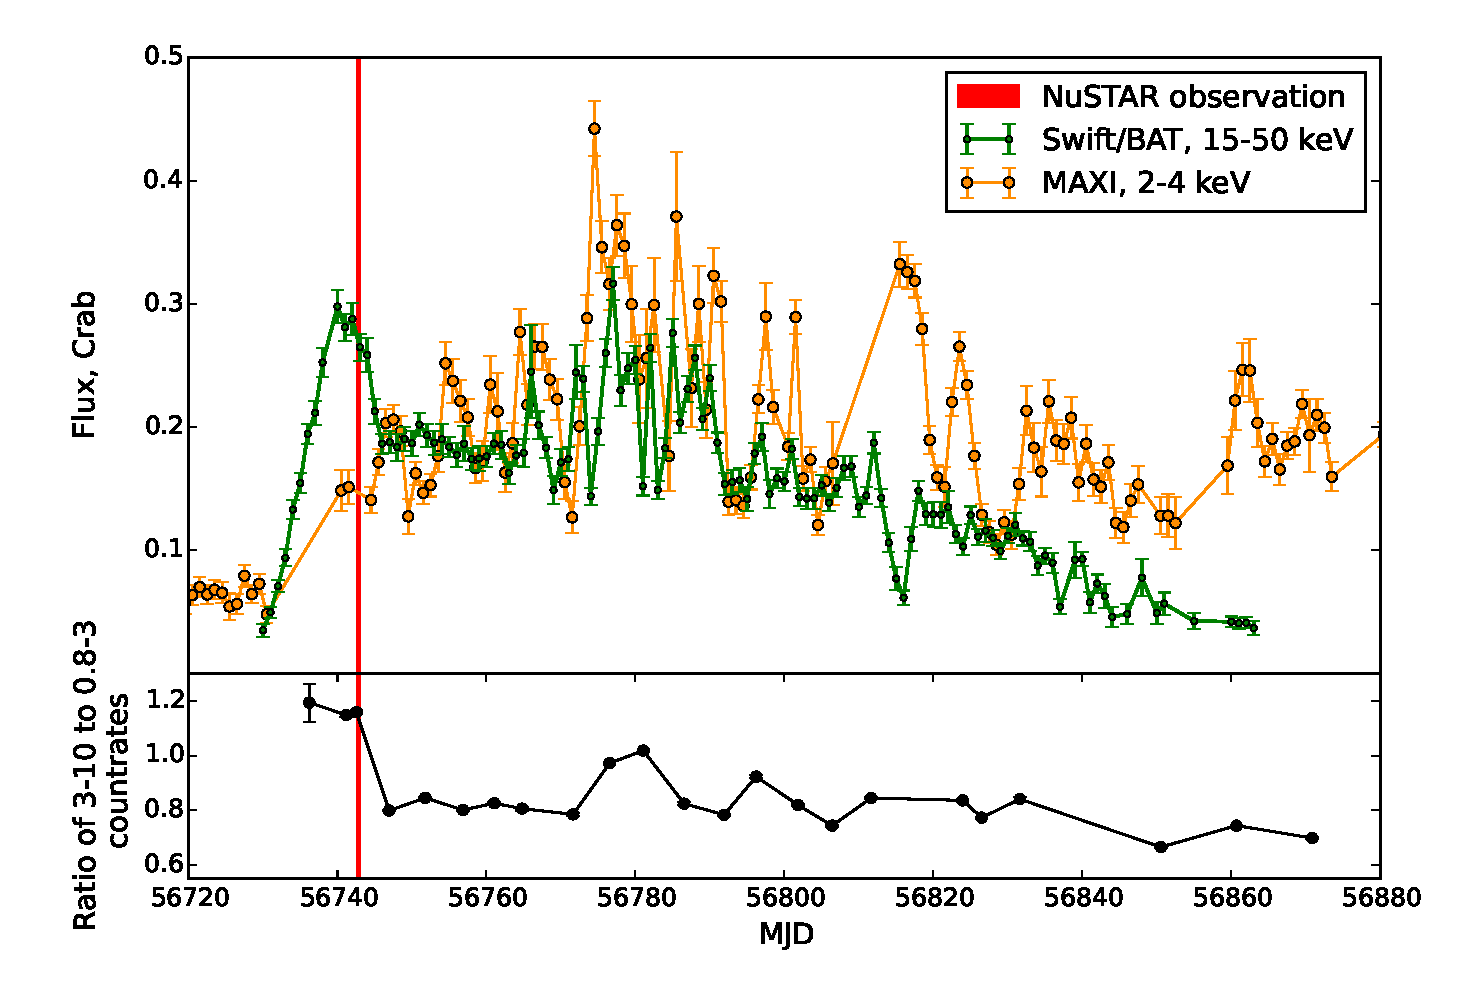
\includegraphics[scale=0.5]{batlc_v06.eps}}
\caption{{\it Upper:} green points denote \swiftb\, lightcurve of 2014 outburst in 15--50~keV range, orange circles correspond to \maxi\, fluxes in 2--4 keV. 
Red line show the time interval of \nustar\, observation. 
{\it Lower:} evolution of \swiftx\, spectral hardness during the outburst.} 
\label{fig:batlc}
\end{figure*} 

\section{Observations and data reduction}
\label{sec:datared} 
In order to characterize the overall outburst profile we used data of \swiftb\, {\it transient monitor} \citep{krimm13bat} in hard X-rays (15--50 keV) as well as data from \maxi\, \citep{matsuoka13maxi} (2--4 keV).

We used \nustar\, observation (ObsID: 80002018002) performed at March 26, 2014 (MJD 56742). 
{\texttt{nuproducts}} pipeline were utilized to extract photons from two-arcminute circular region, centered on the source and to produce lightcurves and spectra.

We also used public observations of \swiftx\, (target ID: 33203) performed regularly over the peak and decline of the outburst.  
Since the source was bright, all \swiftx\, observations were performed in windowed mode, allowing study of timing properties of the source. 
We performed standard analysis with {\texttt{xrtpipeline}} and barycentered data prior to lightcurve extraction. 
During several observations countrate was as high as 280 cts s$^{-1}$, therefore we excluded one or few brightest columns depending on countrate, in order to suppress effects caused by photon pile-up. 
Photons with energies below 0.8 keV and above 10 keV were also filtered out. 
Long-term lightcurves and spectra were obtained from UK Swift Science Data Centre at the University of Leicester \citep{evans09}.

\section{Analysis}
\subsection{Outburst}
First detection of the source by \swiftb\, \citep{krimm14_atel} occurred at March 9, 2014 (MJD 56725, we will refer to this date as $\tau_{0}$). 
Outburst profile in hard X-rays (15--50~keV) featured fast rise with tenfold intensity increasing over ten days, nearly flat-top peak ($\tau_{0}$+10..+15 days) followed by abrupt flux decrease by 30\% over two days.
After this, the source demonstrated gradual decline interrupted by flaring activity at $\tau_{0}$+30..+65 days. 
Another interesting feature is a dip, observed in \swiftb\, lightcurve at $\tau_{0} \approx +86$ days. 
After the cease of the outburst source remained active with flux about 5--15 mCrab. 

Adding data from \maxi\, to the \swiftb\, hard X-ray lightcurve gives us another insight on the outburst evolution as shown in Fig.\,\ref{fig:batlc} - comparing fluxes in soft and hard bands (for 2--4 keV band we took a 1.67 counts s$^{-1}$ as a reference value for Crab, corresponding value for 15--50 keV band is 0.22 cts cm$^{-2}$ s$^{-1}$) one can see that the soft component obviously lags hard emission in the beginning of the outburst but then starts to grow and ends up dominating during the flaring period as well as during hard dip. 
Lower subplot of Fig.\,\ref{fig:batlc} shows evolution of hardness ratio (3--10~keV/0.8--3~keV) measured by \swiftx. 
Right after the peak of hard emission one can see the decline of hardness, also indicating appearance of the thermal component.
For a detailed analysis of the spectral evolution during the outburst see citep[][in preparation]{bykov18}.

Fortunately, \nustar\ observation triggered by \cite{miller15_nust} were carried right at the transition between hard and soft states, thus giving us unique possibility to study processes that happens during HIMS. 

\subsection{NuSTAR observation}
\label{sec:nust} 

\nustar\, observed \grs\ for nearly 30 ks of net exposure right after the hard X-ray peak (see Fig.~\ref{fig:batlc}). 
Earlier, \cite{miller15_nust} shown that the average spectrum of this observation is well described by reflection models such as {\it relxill} \citep{garcia14, dauser14,dauser16} with accretion disk that reaches remarkably close to the black hole innermost stable circular orbit (ISCO), with disk inner edge radius upper estimate being $R_{\rm in} = 5^{+3}_{-4}\, G M/c^{2}$ \citep{miller15_nust}. 
They also noted, that no additional thermal component was needed in order to describe {\it NuSTAR} energy spectrum probably due to the low disk temperature and high absorption.

Given the 96.9 minute orbital period of \nustar, observation is divided in 13 intervals separated by Earth occultations, as shown in Fig.\,\ref{fig:nust_lc}. 
We denoted these intervals with roman numerals, from {\bf I} to {\bf XIII}. 
From the lightcurve of observation it is clear, that the source flux is increasing throughout observation from $\approx$145 up to $\approx$170 counts per second. 
The spectrum also alter, with hardness (defined as ratio of countrates  $R_{3-10\,keV}/R_{10-78\,keV}$) monotonically growing from 2.7 to 3.1. 


\subsubsection{Continuum evolution}
To get better view on the evolution of continuum emission we fitted all individual interval spectra using \texttt{XSPEC} package \citep{arnaud96} with absorbed \texttt{xillver} \citep{garcia13} model (\texttt{const*phabs*xillver}). 
%We peaked {\it xillver} model over the {\it relxill} for separate intervals analysis due to its simplicity and lesser amount of free parameters, since the total number of counts in each interval is not enough to well restrict parameter space of {\it relxill} model.
This model describes reflection of incident radiation from ionized slab of matter. 
The spectrum of incident radiation are assumed to be power-law with exponential cutoff. 
We peaked {\it xillver} model over the {\it relxill} for separate intervals analysis because we wanted to describe the changes in the continuum emission making no assumptions on the system geometry. 

Spectra from two \nustar\, modules of each interval were fitted simultaneously with free cross-calibration constant between modules.
We choose to fix interstellar absorption at $N_{H} = 2.15\times10^{22}$ cm$^{-2}$ as was found by joint \xmm/\nustar\, observation during low luminosity state \citep{fuerst16}. 
Element abundances were taken from \cite{wilms00} and cross-sections from \cite{verner96}. 
Relative iron abundance were fixed at  $A_{Fe} = 1$, ionization parameter at $\xi=3.2$ and inclination at 35 degrees, in consistency with \citet{miller15_nust} results obtained with different spectral models. 
Although in  \texttt{xillver} there is no relativistic broadening of Fe K$\alpha$ emission line no significant residuals in 5--8 keV region are seen, mainly because of limited statistics in per interval spectra. 
Before fitting, spectra were grouped in order to have at least 100 counts per bin, channels above 60 keV were ignored. 
Resulting fits are of satisfactory quality with $\chi^{2}_{red.} \approx 1.05$. 
 
Examination of the best-fit parameters (see Table~\ref{tab:timing} and Fig.\ref{fig:intspe}) confirms that the spectrum softens during the observation and the cut-off energy decreases. 
%Flux is steadily increasing and at the end of the observation unabsorbed luminosity in 3--60 keV band reaches $7\times10^{37}$~erg~s$^{-1}$ for 8 kpc distance. 

\subsubsection{Constrains on movement of the inner parts of accretion disk}
Spectra of single intervals have not enough statistics to constrain change of Fe-line profile and, hence, to determine whether the disk inner boundary  is moving during observation. 
To increase statistics, we split whole observation into three major pieces, with first made by intervals {\bf I-IV}, second by {\bf V-IX} and third by {\bf X-XIII} and extracted 4--78 keV spectra. 
We chose to group them in order to have at least 100 counts per bin and then we fitted them (excluding data between 5--10 keV) with simple \texttt{phabs*cutoffpl} model, using, once again, $N_{H} = 2.15\times10^{22}$ cm$^{-2}$.  

Now, plotting the ratio of this fit to initial spectra (see Fig.~\ref{fig:ratios}) one can see that both strong features - i.e. Fe-line complex at 5--9 keV and Compton hump around 30 keV are seemingly stable. 
Therefore we can conclude, that there is no drastic change in position of inner disk boundary between parts of observation. 
Additionally, we estimated the equivalent width of  Fe K$\alpha$ emission line in this three parts - we approximated 4--78~keV spectra with 10--30~keV range being ignored (to neglect the Compton-hump contribution) with model consisting of absorbed cut-off powerlaw and gaussian. 
Equivalent width of the gaussian component is around 0.175 keV and remains constant along the observation within error margins, although it is possible that the quality of data is not enough to trace the real change.

\begin{figure*}
\centerline{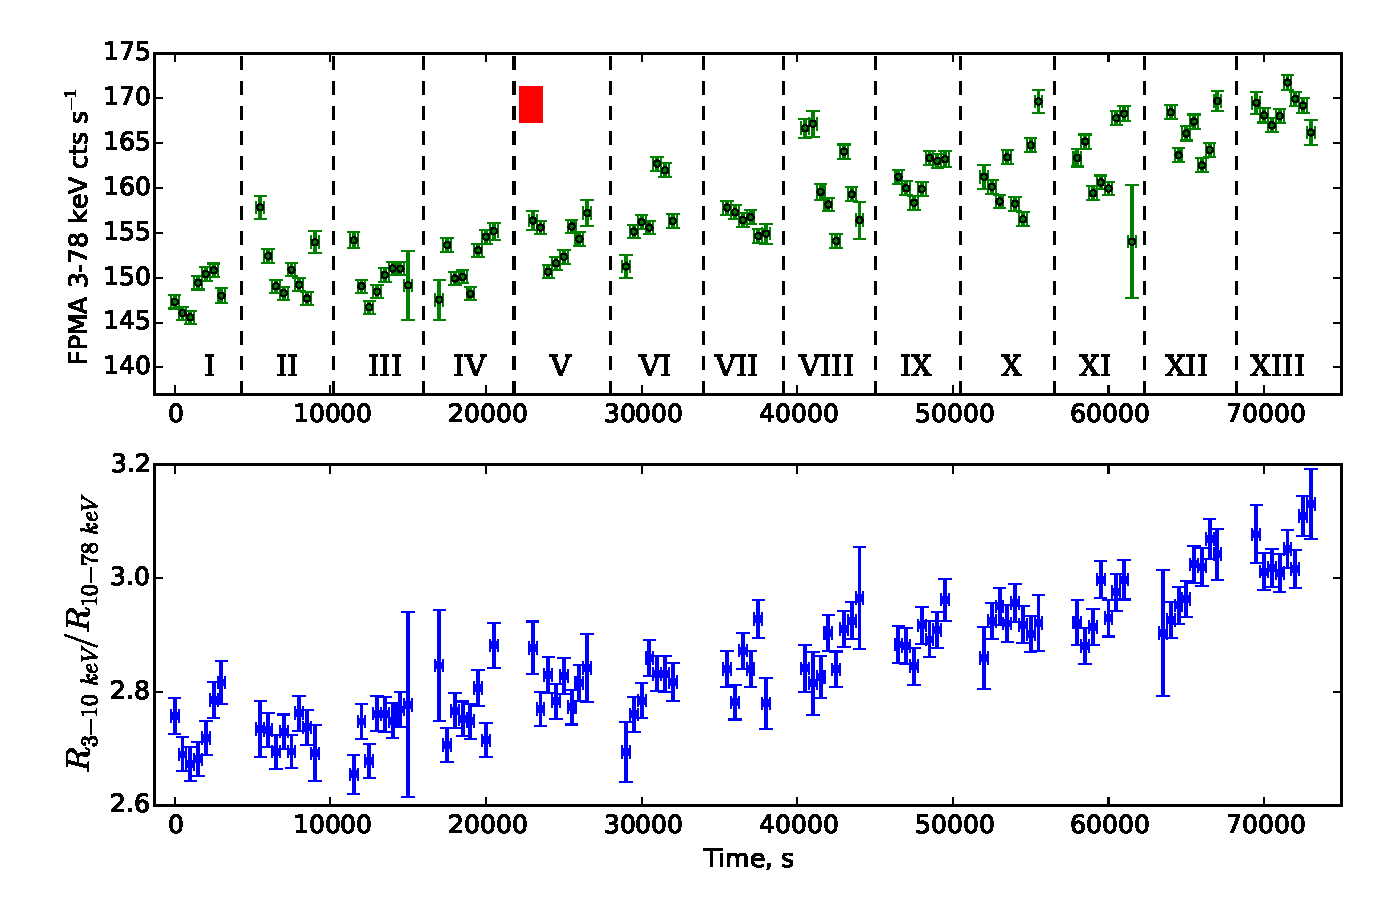
\includegraphics[scale=0.7]{nuAlc_color_v04.eps}}
\caption{Upper panel: countrate of \nustar\,FPMA in 3--78 keV band. We enumerated intervals of uninterrupted observations with roman numerals. Red square shows time of simultaneous \swiftx observation (ObsId: 00033203003, second part). Bottom panel: evolution of hardness during observation} 
\label{fig:nust_lc}
\end{figure*} 
 \begin{figure}
\centerline{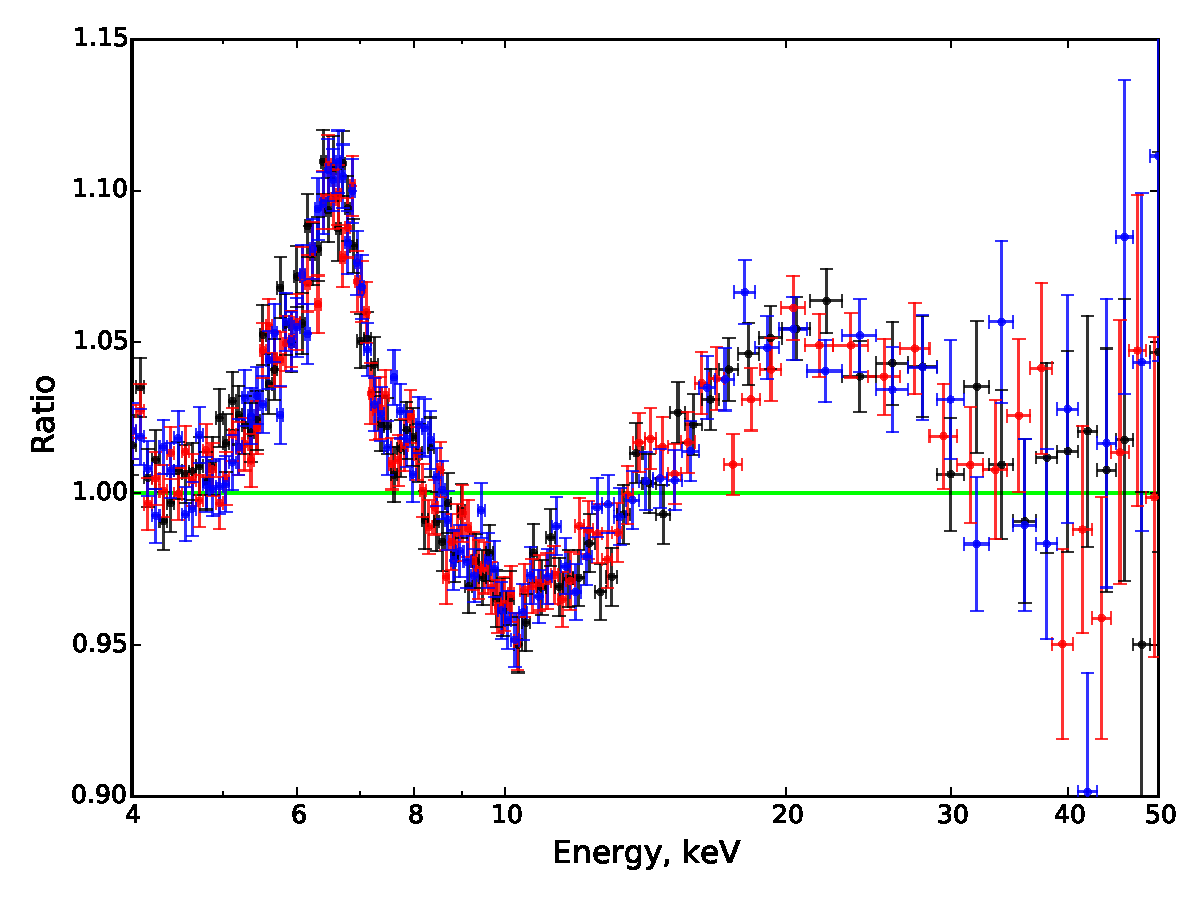
\includegraphics[width=\linewidth]{ratios_v01.pdf}}
\caption{Ratio of \nustar\, FMPA spectra to \texttt{phabs*cutoffpl} model. In black - data from intervals I-IV, in red from V-IX and in blue from X-XIII.} 
\label{fig:ratios}
\end{figure}  

\begin{figure}
\centerline{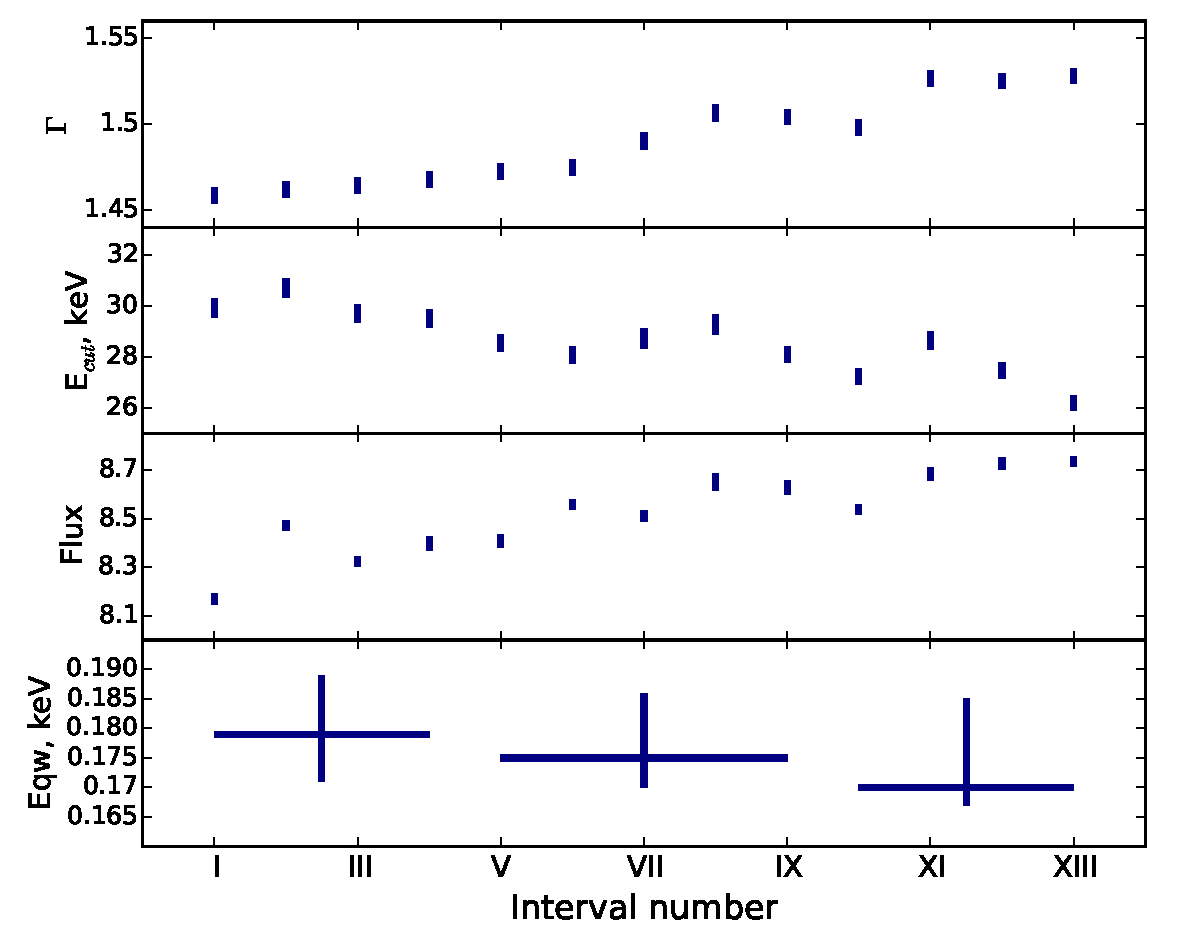
\includegraphics[width=\linewidth]{intspe_v04.eps}}
\caption{Parameters of continuum emission in intervals. From upper to lower: \texttt{xillver} powerlaw slope, cutoff energy,  flux in 3--60 keV band $\times$\, erg s$^{-1}$ cm$^{-2}$ and Fe-line equivalent width.} 
\label{fig:intspe}
\end{figure}  
            
\subsubsection{Average spectrum analysis}
\label{sec:spec}            
There is a 1.3 ks part of \swiftx\, snapshot (ObsId: 00033203003) that coincides with \nustar\, observation. 
Extension of an energy range to 0.8--78 keV allows one to search for thermal emission associated with the cold inner disk with $kT \sim 0.1...0.4$~keV (such as were found in other BHCs, see \cite[][ e.t.c]{miller06b,miller06a,parker15}).

We extracted \swiftx\, spectrum using only zero-grade events, grouped it to has at least 30 counts per bin and added 3\% systematic error. 
Similar grouping were applied to \nustar\, data. 

Since the average spectrum has much better statistics we will apply more sophisticated {\it relxilllp} spectral model that describes reflection of emission produced by point source located on the rotation axis above the Kerr black hole from the relativistic accretion disk. 
We used latest available version of {\it relxilllp} package (v1.0.2).
Jet foundation are often thought to be responsible for this type of ``lamp-post'' geometry. 
Among the parameters of a model several are of a particular interest, namely $h$ - height of a point source above the black hole illumination the accretion disk and $R_{in}$ - its inner radius.  
We selected this model for several reasons - first, \cite{miller15_nust} found that it matches {\it NuSTAR} data well. 
Also, during the 1996 outburst source was detected at radiowaves, possibly indicating jet activity. 
For spectral fitting we used \texttt{migrad} minimizer from {\em MINUIT} package \citep{james75minuit}, and in order to estimate errors we employed a large MCMC chain. 

Interestingly, instead of surplus thermal component we found a lack of the soft emission - usage of $N_{H} = 2.15\times10^{22}$ cm$^{-2}$, measured in the low state \citep{fuerst16_gx339} led to worse fits with systematic negative residuals below few keV. 
Therefore, we left $N_{H}$ free during the fit. 
Obtained value of 2.6$\times10^{22}$ cm$^{-2}$ is higher than one measured by \cite{fuerst16_gx339}. 
This can be possibly accounted to a presence of disk outflow, caused by severe X-ray irradiation. 

Obtained upper limit on truncation radius of accretion disk - $r_{in} < 9 GM/c^{2}$ (90\% confidence limit) is similar to the value from \cite{miller15_nust}, height of the source above the accretion disk is in agreement too. 
Some discrepancy seen in the parameters of accretion disk - e.g. inclination, ionization parameter and Fe-abundance, it can be caused by broader energy range. 
As it can be seen from Fig.~\ref{fig:spec} there is no significant residuals in lower-energy part of the spectrum, therefore thermal emission from accretion disk is too weak or too cold to detect. 

Total unabsorbed flux in 0.1--100 keV band is about 1.4$\times$10$^{-8}$~erg s$^{-1}$ cm$^{-2}$ which translates to a luminosity of 1.1$\times$10$^{38}$ erg s$^{-1}$ for the 8 kpc distance. 
Typical luminosity at which BHCs change from LHS to HIMS is about $0.1 L_{Edd} = 1.2\times10^{37} (M/M_{\odot})$ erg s$^{-1}$, although we should note that there is significant scatter in this value. 
Therefore one can put a rough lower estimate on the black-hole mass as 9 $M_{\odot}$, which is reasonable.

\begin{table}
\noindent
\centering
\caption{Best-fit parameters of \texttt{phabs*relxilllp} model}
\label{tab:fullfit}
\centering
\begin{tabular}{|c|c|}
\hline\hline
Parameter & Value \\
\hline
$N_{H}, 10^{22} cm^{-2}$ &   2.64$^{+0.05}_{-0.03}$ \\   
$h, GM/c^{2}$   &  22.3$^{+0.6}_{-4.3}$ \\
$a, cJ/GM^{2}$    & 0.73$^{+0.26}_{-0.23}$   \\
$incl, deg$ & 22.1$^{+2.9}_{-2.0}$ \\
$R_{in}, ISCO$  & 1.05$^{+1.73}_{-0.02}$ \\ 
$\Gamma$& 1.40$^{+0.01}_{-0.01}$   \\
$\log{\xi}$ &  3.52$^{+0.05}_{-0.07}$ \\
$A_{Fe}$   &  3.0$^{+0.6}_{-0.3}$  \\        
$E_{cut}, keV$    &       26.3 $^{+0.3}_{-0.5}$    \\
$R_{refl}$  &         0.42$^{+0.03}_{-0.03}$    \\
$N_{FMPA},\,\times10^{-2}$          &      1.49$^{+0.09}_{-0.03}$ \\
$C_{FMPB}$ & 1.017$^{+0.002}_{-0.001}$    \\
$C_{Swift-XRT}$    &   1.04$^{+0.01}_{-0.01}$\\
$\chi^{2}_{red.}$    &   1.1=\\ 
              &= 3366.21/3062 d.o.f\\
              
\hline
\end{tabular}
\end{table}




\begin{figure}
\centerline{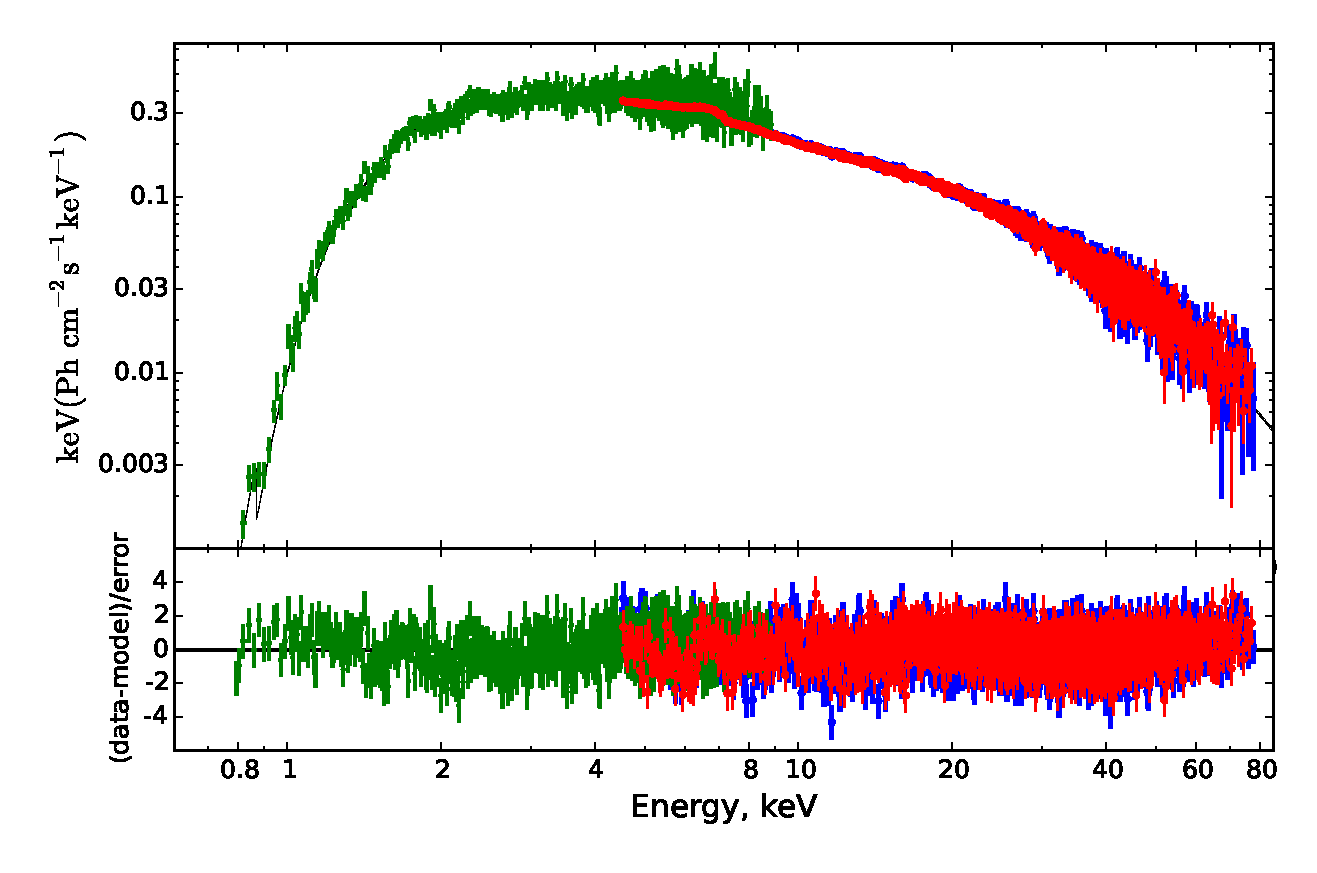
\includegraphics[width=\linewidth]{spectrumfit_v02.eps}}
\caption{Fit of composite \swiftx/\nustar spectrum by \texttt{phabs*relxilllp} model. Green, red and blue points correspond to \swiftx, \nustar FPMA and FPMB, correspondingly.} 
\label{fig:spec}
\end{figure}  


\section{Timing analysis} 
%    Along with the spectral analysis of X-ray transients, timing analysis give a vast of information about the geometry and current state of the accretion flows in such systems. 
%For example, broad band timing variability properties are used in determination of the systems state \cite{2005Ap&SS.300..107H}.
%
%    Variability properties of different types of X-ray binary systems are usually described in terms of the luminosity power spectrum, which is a common technique on determination of amount of power in the particular frequency range.
%    Luminosity variability power spectrum of the transient system typically can be described with a set of broad and thin Lorentzian functions representing correspondingly broad band stochastic noise and QPOs \citep[see, e.g.][]{1972ApJ...174L..35T, 1990A&A...227L..33B}.
%    The overall variability and the shape of the power spectrum changes dramatically with the spectral states of the transients and, in some cases, manifest state transitions even if they are not evident from the energy spectrum.
%
%    Some aspects of the evolution of the X-ray binaries system power spectrum with their state can be explained in the frame of the two-temperature accretion flow model, where it consists of the geometrically thin cold disk and geometrically thick hot flow (corona), particularly it is widely accepted that the high amplitude variability is associated with the geometrically thick flow, while the geometrically thin disk is generally stable \citep{2001MNRAS.321..759C}. 
%It should be noted that this model of the variability generation are directly connected with the models, explaining energy spectra of black hole binaries \citep[see, e.g.,][]{1975ApJ...199L.153E, 1976ApJ...204..187S, 1995ApJ...452..710N}, \citet{2001MNRAS.321..759C} has shown with the frequency resolved spectroscopy that variable part of the emission has a hard spectrum, which is thought to be produced in the corona, while stable part of the emission has a spectrum which is consistent with the cold classical $\alpha$-disc spectrum \citep{ss73}.
%
%    It is generally accepted that the broadband noise observed in the power spectrum of binary systems is produced due to the stochastic variations of the angular momentum transport efficiency \citep{1997MNRAS.292..679L}. 
%    In this propagating fluctuation model broad band noise is a product of noisy signals from different radii of the accretion flow, each with its own characteristic time-scale \citep[see, e.g.][]{2006MNRAS.367..801A, 2013MNRAS.434.1476I}.
%    It follows, that the shape of the broad band noise is determined with the physical and geometrical properties of the accretion flow, e.g. in particular in these works it was suggested that the broad noise dumping frequency is connected to the accretion flow inner edge.
%
%    Another feature, frequently observed in the X-ray binaries power spectra is different types of low and high frequency QPOs manifesting itself as an excessive power in the thing frequency bands. 
%    There is at least five types of these QPOs were observed on the frequencies above 0.1~Hz in the stellar mass binary systems \citep[for classification see][]{2005Ap&SS.300..107H}.
%
%Several models were proposed to explain high and low frequency QPO features in power spectra \citep[][]{1997ApJ...489..865E, 1998ApJ...506..281B, 1998ApJ...492L..59S, 1999A&A...349.1003T, 1999ApJ...518L..95T, 2001A&A...374L..19A, 2009MNRAS.397L.101I, 2011MNRAS.415.2323I}. 
%Changes, observed with the evolution of the spectral states between different types QPOs and broad band noise, e.g. correlation between QPOs centroid frequencies and broad noise dumping frequency \citep{1999ApJ...514..939W, 2014MNRAS.437.2554M} speak in favor of the origin of the QPOs in the inner edge of the accretion flow.
%
%While these models, describing broad band noise and QPOs in the variability power spectrum, usually do not confront observed energy spectra, it was found that some additional demands on time properties must be met.
%\citet{1997ApJ...474L..43V} used coherence spectrum in order to additionally constrain time properties of the accretion flow. 
%They found a time lag between hard and soft emission of the soft and hard emission, which have a complex behaviour with the frequency, which they used to constrain geometrical size of the accretion flow \citep{1999ApJ...517..355N}. 
%Observed time lags also were used to discriminate some spectral models \citep[see, e.g.,][]{2001MNRAS.327..799K}.

Variability properties of different types of X-ray binary systems are usually described in terms of the power spectrum.
%, which is a common technique for determination of amount of power in the particular frequency range. 
Power spectrum of the BHC systems in LHS typically can be described as a combination of a band-limited noise and one or few narrow Lorentzian functions, representing QPOs \citep[see, e.g.][e.t.c]{1972ApJ...174L..35T, 1990A&A...227L..33B, homan05}. 
Properties of this components and correlations between them, in principle, may be used to discriminate between different models, proposed for generation of X-ray emission in BHC. 
 
Although power spectra analysis is by far the most popular, more sophisticated methods, such as coherence function or phase-lag were successfully used to infer physical properties of accretion flows. 
Using a measured time-lag between the soft and hard emission, which has a complex behavior with the frequency \citet{1999ApJ...517..355N} constrained geometrical size of the accretion flow. 

%\citet{1997ApJ...474L..43V} used coherence spectrum in order to additionally constrain time properties of the accretion flow. 
%They found a time lag between hard and soft emission of the soft and hard emission, which have a complex behavior with the frequency, which they used to constrain geometrical size of the accretion flow \citep{1999ApJ...517..355N}. 
%Observed time lags also were used to discriminate some spectral models \citep[see, e.g.,][]{2001MNRAS.327..799K}.

In the following section we present analysis of the \grs\ timing properties and their evolution during the 2014 outburst.

\subsection{Power spectrum}

We split {\it NuSTAR} observation of the \grs\ 2014 outburst on 13 continuous intervals separated with $\sim0.7$~hr intervals when the source was occulted by Earth. 
The continuous intervals have duration from $\sim2440$ to $\sim3390$~sec see Table~\ref{tab:timing}.
Since {\it NuSTAR} detectors operate in the photons counting mode, data can be reduced to the light-curve with time resolution up to 2$\mu$s.
For our analysis we extracted light-curves with 0.01~s temporal resolution in a few energy bands (3--78, 3--10, 3--5, 5--8, 8--15, 15--78, 10--78~keV), which allows us to examine $\sim3\times10^{-3}$--$50$~Hz frequency range.
As it was mentioned above, this is a frequency band which usually contains low frequency QPOs and broad band noise \citep{wijnands99}.

{\it NuSTAR} detectors are subject to non-paralyzing dead time with characteristic timescale $\tau \approx 2.5$~$\mu$s \citep{2015ApJ...800..109B}, in our case the effects from dead-time are already present at frequencies above 20~Hz.
\citet{2015ApJ...800..109B} noted that {\it NuSTAR} dead-time has a complex dependence on the energy of registered photons, and therefore it is hard to create analytical model for resulting power spectra. 
They proposed to use the real part of the cross spectrum of light-curves obtained from two {\it NuSTAR} detectors for the estimation of the power spectrum 
\begin{equation}
        re(F_{\rm FPMA}^{*}F_{\rm FPMA})
\end{equation}
where $F_{\rm FPMA[B]}$ - Fourier function of a light curve from FPMA[B] module, $^{*}$ - stands for complex conjugation. 

This method is based on the following assumption: signals produced by an observed source on two detectors are identical and have no time lag and therefore their Fourier functions are also identical and have zero phase shift, in contrast, signals independent for two detectors (like counting statistics) have random phase shifts.  
It follows that for independent signals the average real part of the cross spectrum tends to zero due to the random phase shift .

\citet{2017arXiv170909666H} shown that the cross-spectrum (or shortly cospectum) in each frequency bin is distributed with Laplace probability density function (PDF) if it is derived from two normally distributed random independent series \citep[see, e.q. 14 in ][]{2017arXiv170909666H}:
\begin{equation}
        p(C_{j}|0, \sigma_x \sigma_y) = \frac{1}{\sigma_x \sigma_y} exp{\left(\frac{-|C_{j}|}{\sigma_x \sigma_y} \right)}
\end{equation}
Where $C_{j}$ - cospectrum of two {\it uncoherent} series measured in the $j$-th frequency channel and $\sigma_x$, $\sigma_y$ - are second momenta of the initial normal distributions (therefore they are equal to the square of the power spectra in corresponding frequency channel for each time series).
If signals used for the cospectrum estimation have identical power spectra then $\sigma_x = \sigma_y \approx |F_{\rm FPMA}|$.
We, therefore, see that to determine proper likelihood function which can be used to approximate cospectra with analytical functions, one still has to know Poisson noise level.
It is also worth noting, that source countrate and total countrate are usually slightly differs for two {\it NuSTAR} modules making amplitudes of counting-statistic and dead-time not equal.
Taking all this arguments into consideration we decided to use standard power spectrum for our analysis.

Since we used relatively large time bining (10 ms) to extract lightcurves from {\it NuSTAR} data and also usually considered variability at frequencies below 10~Hz, we assumed that the only effect from the dead-time is lowering of the constant Poisson noise level on the $(1 - 2\nu \tau_{\rm d})$ factor, where $\nu$ is total count rate for detector and $\tau_{\rm d}$ is a dead time \citep{1994A&A...287...73V, 1995ApJ...449..930Z}. 
Since the dead-time is not constant along energy band, we measured modified Poisson level for each extracted data-set separately.
%To simplify our analysis we decide to use standard 
%We therefore decided to use power spectrum for the intrinsic variability estimation.
%To simplify our analysis we inspect power spectrum only on frequencies below 10~Hz.

%%!!!!

Power spectrum of each of separate interval of {\it NuSTAR} observations has a form of a white noise plateau ($P(f)\propto const$) on the low frequencies, transforming at the frequency $\approx0.1$~Hz in to the power law with the slope $\rho\approx-1.6$..$-2.0$. 
Also a prominent QPO at the frequencies 0.3--0.7~Hz and its second harmonic are present. 
Typical power spectrum of a single interval is shown in Fig.~\ref{fig:qpo}.
From the shape of the energy and Fourier spectrum we concluded that the system is in the hard intermediate state and observed low frequency QPO (LF QPO) is of type C. 

For the light-curves extracted in 3--78~keV energy range Poisson noise dominates intrinsic source variability on the frequencies over $\approx1$~Hz, preventing analysis of any high-frequency features.
There is also signs that the Power spectrum on the frequencies below $\approx0.003$~Hz has a form of growing power law $P(f)\propto f^{\alpha}$, $\alpha > 0.3$.
We did not try to find any high frequency QPOs, since the typical HF QPO (centroid frequency 100-400~Hz, amplitude $\approx10$\% and quality $Q\approx2$--$10$) is indiscernible over the Poisson noise with the obtained count-rate and duration of the observation.


%To track the source variability evolution we fitting relatively short observations with duration of 2--3~ks, and therefore can not split them on more than few dozens parts in order to have an eye on the power spectrum break feature on the 0.1~Hz frequency. 

In order to assess properties of \grs\ intrinsic variability we approximate each obtained power spectra with the following analytical function:
\begin{equation}
        \begin{aligned}
                P(f)  = & n (1 + (f/f_{\rm lb})^4)^{\alpha} + \\
                     &\frac{s_1}{(f - f_{\rm QPO})^2 + (f_{\rm QPO}/Q_{\rm m})^2} +\\
                        & \frac{s_2}{(f - 2f_{QPO})^2 + (2f_{\rm QPO}/Q_{\rm m})^2} + \\
                        & poiss
\end{aligned}
        \label{eq:complex_fit}
\end{equation}
Where $f_{\rm lb}$ - broad noise break frequency, $f_{\rm QPO}$ and $Q_{\rm m}$ - centroid of the QPO and its quality correspondingly and poiss - represents mean power of the variations caused by the counting statistics and dumped by dead-time.
In this function first component represents plateau with the break, second two components describe QPO main harmonics and its overtone, last component represents constant Poisson noise.
We take that the quality of the QPO harmonic is equal to the QPO peak quality.
Further in the text will mention this models as standard.

\begin{figure}
        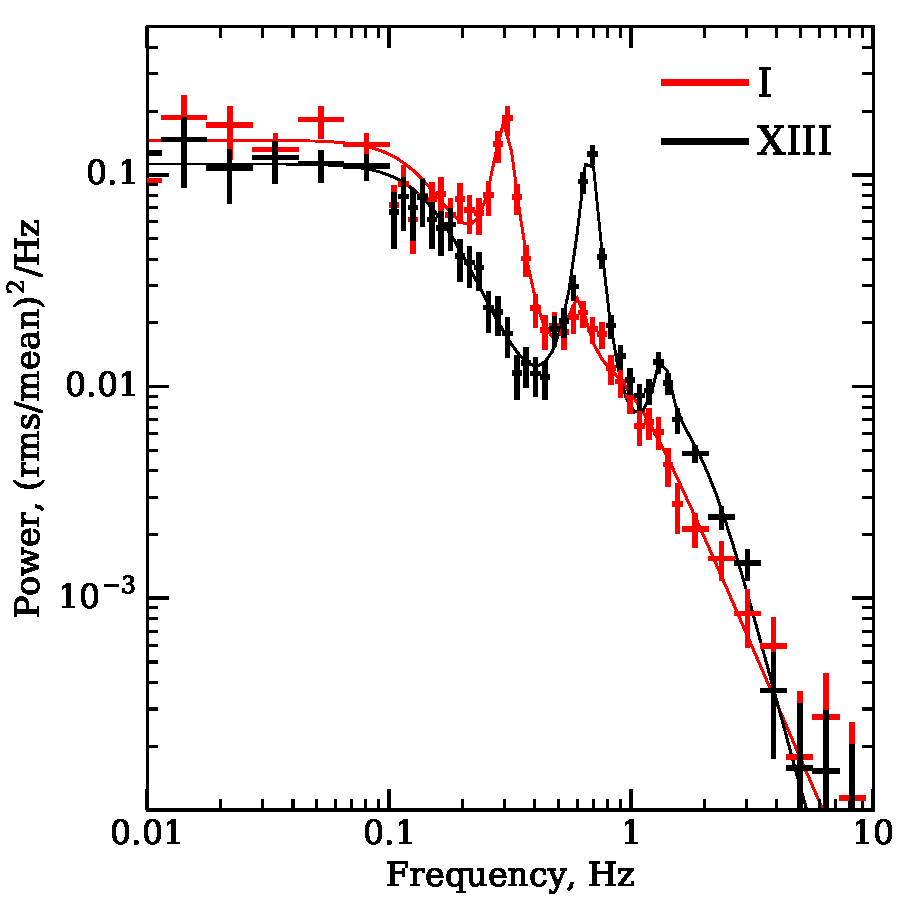
\includegraphics[width=\columnwidth]{qpo_centroid_evolution.pdf}
        \caption{Power spectrum of the \grs\ obtained with {\it NuSTAR} data at the beginning (red crosses) and at the end (black crosses) of the observation. Poisson noise is subtracted.}
        \label{fig:qpo}
\end{figure}


We found that the QPO frequency had clearly evolved with time see Table~\ref{tab:timing} and Figure~\ref{fig:qpo}.
The QPO frequency correlates with the {\it NuSTAR} flux and photon index, similar to many other black hole and neutron star binary systems \citep[see, e.g.,][]{vignarca03,2003A&A...407.1039P}.
On the other hand we see, that the QPO amplitude remained stable during the first half of the observation, and started to grow in the second part.

\begin{table*}
\noindent
\centering
\caption{Evolution of the Fourier and energy spectrum properties through the {\it NuSTAR} observation in the 3--78~keV energy band.}
\label{tab:timing}
\centering
\begin{tabular}{|c|c|c|c|c|c|c|c|c|c|c|}
\hline\hline
Interval    & T$_{start}$,  & Expo,     & f$_{\rm br}$,                     & f$_{\rm QPO}$, & Q$_{\rm m}$,     & A$_{\rm m}$,  & A$_{\rm o}$,      & rms & $\Gamma$ & E$_{\rm cut}$, \\
            &  MJD          &  s        & $\times10^{-2}$, Hz               &  Hz            &   & \%            &  \%               &   \%       &          &  keV             \\
\hline
I           & 56742.68      & 3386      & $8.9_{-2.3}^{+2.2}$  & $0.30\pm0.01$ & $15_{-3}^{+5}$ & $7.5_{-1.0}^{+0.9}$ & $2.7_{-0.9}^{+0.8}$ & $26\pm1$ & $1.459\pm0.005$ & $29.9\pm0.4$ \\
II & 56742.75 & 3388 & $7.8_{-1.8}^{+2.0}$ & $0.31\pm0.01$ & $13\pm3$ & $7.9_{-0.9}^{+1.0}$ & $2.7_{-0.9}^{+0.8}$ & $26\pm1$ & $1.462\pm0.005$ & $30.7\pm0.4$ \\
III & 56742.82 & 3392 & $8.2_{-1.9}^{+2.4}$ & $0.34\pm0.01$ & $12_{-2}^{+3}$ & $7.7_{-0.8}^{+0.9}$ & $3.9_{-0.8}^{+0.9}$ & $26\pm1$ & $1.464\pm0.005$ & $29.7\pm0.4$ \\
IV & 56742.88 & 3389 & $8.3_{-1.8}^{+2.0}$ & $0.35\pm0.01$ & $15_{-3}^{+4}$ & $7.6\pm0.9$ & $3.2_{-0.8}^{+0.7}$ & $26\pm1$ & $1.468\pm0.005$ & $29.5_{-0.3}^{+0.4}$ \\
V & 56742.95 & 3389 & $6.9_{-1.4}^{+1.6}$ & $0.39\pm0.01$ & $13_{-3}^{+4}$ & $7.4\pm0.8$ & $4.3_{-0.9}^{+0.8}$ & $26\pm1$ & $1.473\pm0.005$ & $28.6\pm0.3$ \\
VI & 56743.02 & 3136 & $7.5_{-1.5}^{+1.9}$ & $0.41\pm0.01$ & $17_{-3}^{+5}$ & $6.9_{-0.8}^{+0.9}$ & $3.8_{-0.8}^{+0.7}$ & $26\pm1$ & $1.475\pm0.005$ & $28.1\pm0.3$ \\
VII & 56743.09 & 2771 & $9.7_{-2.2}^{+2.7}$ & $0.43\pm0.01$ & $12_{-2}^{+3}$ & $7.4\pm0.9$ & $3.6\pm0.9$ & $26_{-1}^{+2}$ & $1.500\pm0.005$ & $28.7\pm0.4$ \\
VIII & 56743.15 & 3387 & $5.8_{-1.5}^{+1.4}$ & $0.46\pm0.01$ & $11_{-2}^{+3}$ & $7.9\pm0.9$ & $4.2_{-0.8}^{+0.9}$ & $27\pm2$ & $1.507\pm0.005$ & $29.3\pm0.4$ \\
IX & 56743.22 & 3392 & $7.1_{-1.4}^{+1.6}$ & $0.50\pm0.01$ & $12_{-2}^{+4}$ & $7.9\pm0.8$ & $4.3\pm0.8$ & $26\pm1$ & $1.504\pm0.005$ & $28.1\pm0.3$ \\
X & 56743.29 & 3390 & $7.0_{-1.6}^{+1.7}$ & $0.53\pm0.01$ & $13_{-2}^{+3}$ & $8.7\pm0.7$ & $4.5_{-0.8}^{+0.7}$ & $25\pm1$ & $1.498\pm0.005$ & $27.2\pm0.3$ \\
XI & 56743.35 & 3382 & $(6.7\pm1.5)$ & $0.57\pm0.01$ & $13\pm3$ & $9.1_{-0.7}^{+0.8}$ & $4.0\pm0.8$ & $25\pm1$ & $1.527_{-0.005}^{+0.004}$ & $28.7\pm0.3$ \\
XII & 56743.42 & 3386 & $6.7_{-1.4}^{+1.8}$ & $0.63\pm0.01$ & $14_{-2}^{+3}$ & $9.5_{-0.7}^{+0.8}$ & $4.4\pm0.7$ & $26_{-1}^{+2}$ & $1.525\pm0.004$ & $27.5\pm0.3$ \\
XIII & 56743.49 & 3391 & $7.5_{-1.5}^{+1.7}$ & $0.67\pm0.01$ & $15\pm3$ & $9.6\pm0.7$ & $4.2\pm0.8$ & $25_{-1}^{+2}$ & $1.528\pm0.004$ & $26.2\pm0.3$ \\
\hline
\end{tabular}
\end{table*}

%Some models suggest that type-C QPO arise due to the Lense-Thirring precession of the accretion flow inner parts \citep{stella98, 2006ApJ...642..420S, ingram09}.
%In such models growth of the QPO frequency corresponds to the shrinking of the disk inner radius.
%However, sophisticated spectral models applied to the observed {\it NuSTAR} spectrum suggest that the accretion disk inner radius was $R_{\rm in}<9 GM/c^2$ during the observation.
%This estimation is primarily based on the profile of the relativistically widened neutral Iron fluorescent line, see section~\ref{sec:spec} and also \citet{miller15_nust}.

We found that the QPO amplitude is smaller in the soft band, while amplitude of it's harmonic is bigger.
The ratio of the power in the QPO and its harmonic for hard and soft energy bands is presented in Fig.~\ref{fig:qpo_ratio}.
\begin{figure}
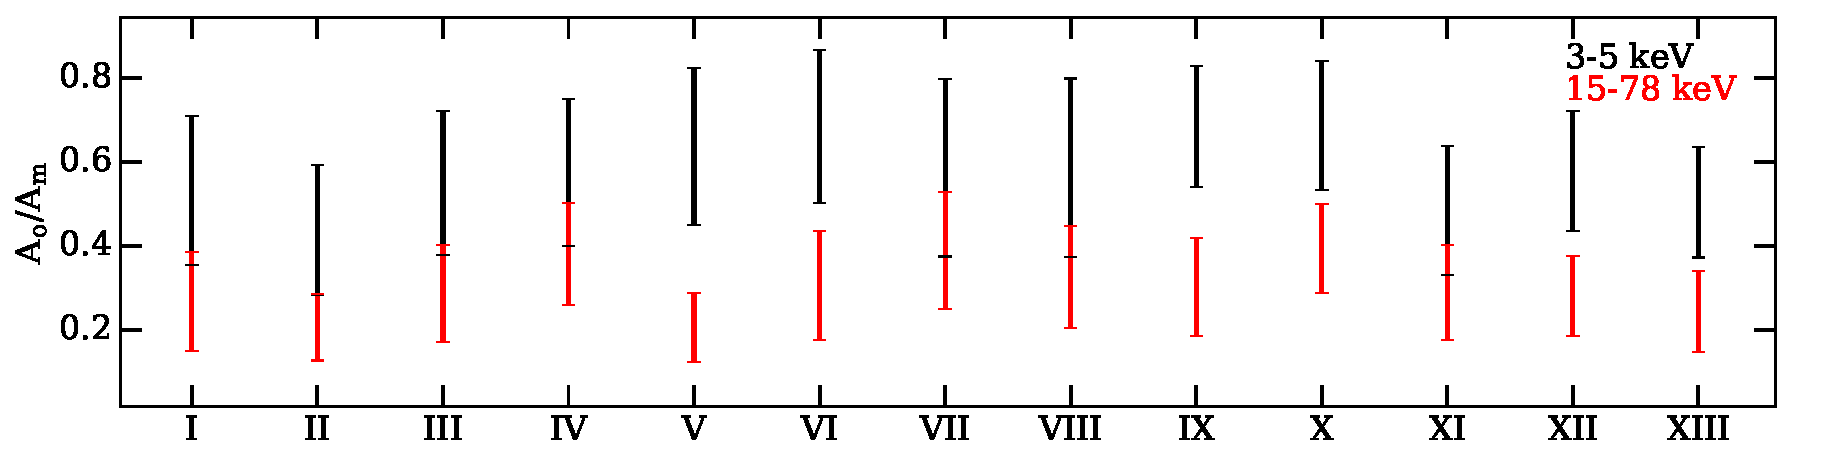
\includegraphics[width=\columnwidth]{QPO_and_harmonic_ratio_ylabel.pdf}
        \caption{Ratio of the total power in the QPO and its second harmonic measured for the lightcurves obtained in 3--5~keV and 15--78~keV energy bands.}
        \label{fig:qpo_ratio}
\end{figure}
It follows that the QPO profile, if it is present \citep[see, e.g.][]{2015MNRAS.446.3516I}, differs in the hard and soft X-ray bands.
Following \citep{2015MNRAS.446.3516I} we tried to extract QPO profile segregating the coherent part (Fourier signal with conserving phase shift relative to the signal on QPO frequency) between the QPO and its harmonics, however no significant coherence was presented above the noise level.
It indicates that the QPO profile was not stable during the observation, in contradiction to the result obtained by \citet{2015MNRAS.446.3516I} for GRS~1915+105 with {\it RXTE} observatory data.


In some intervals QPO subharmonics, centered approximately at the 1/2 of the QPO centroid frequency, is clearly observed in the cospectra (see examples on Fig.~\ref{fig:cospec_tracked}, red crosses) (namely I, II, IV, V, VI sets).
In order to observe QPO with better significance we stacked several cospectra, frequency of each cospectrum was scaled in such a way to conserve QPO centroid at 0.3~Hz.
Obtained ``tracked'' cospectrum is presented on Fig.~\ref{fig:cospec_tracked}.
The subharmonics seems to roam around the 1/2 QPO frequency, therefore we were not able to obtain it with a large significance on the tracked cospectrum.


\begin{figure}
        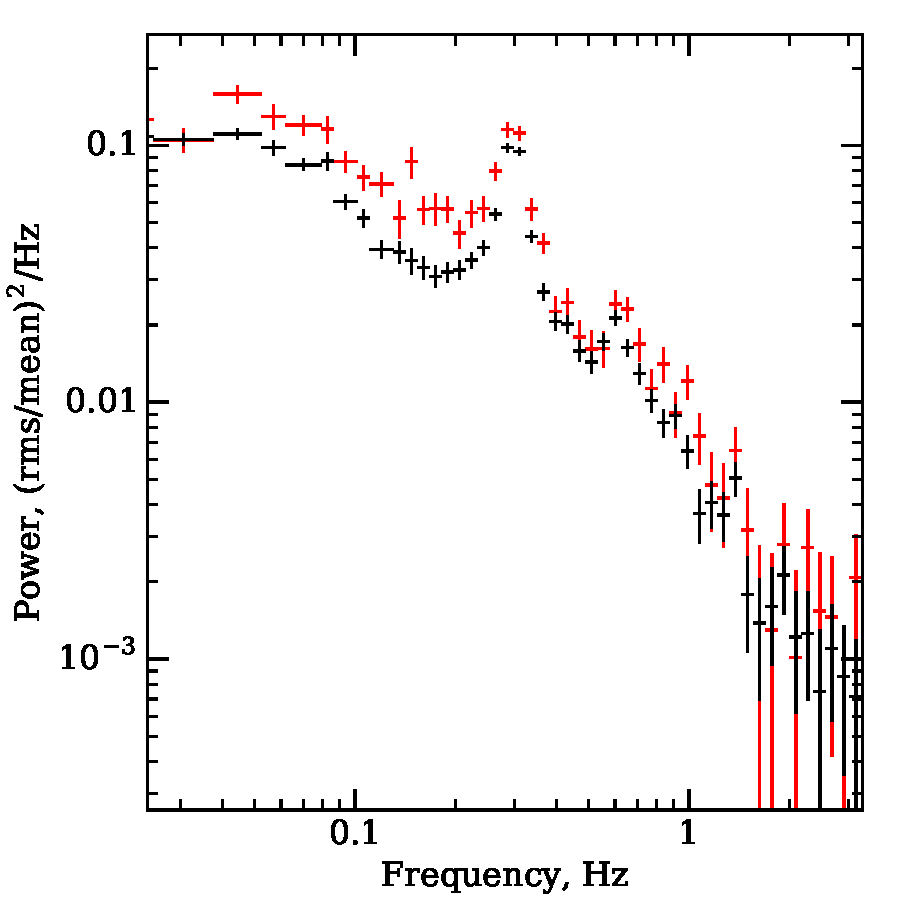
\includegraphics[width=\columnwidth]{folded_cospectr2.pdf}
        \caption{Cross-spectrum of the observations, obtained by scaling frequency to conserve QPO position.
        Black crosses obtained from the all intervals, while red crosses are from intervals I, II, IV, and V, in which QPO subharmonics was most prominent.}
        \label{fig:cospec_tracked}
\end{figure}

It should be noted that the changes in the QPO centroid position during the interval may contribute to the observed quality factor $Q$.
We can estimate the derivative of the QPO centroid position with time (by approximating $f_{\rm QPO}(time)$ with the straight line), which appears to be $\dot{f}_{\rm QPO} \approx 5.0$--$6.5\times10^{-6}$~Hz~s$^{-1}$. 
During an interval with the duration $\tau = 3000$~s observed QPO drift will broaden the perfect periodic signal located at $f_{\rm QPO}=0.3$~Hz up to the quality factor $Q \approx f{\rm QPO}/(\dot{f_{\rm QPO}}\tau) \approx 17$, which is of order of the Q estimations obtained from the observations with standard model (described with eq.\ref{eq:complex_fit}).
In order to better estimate the QPO quality factor, we split each of the 13 intervals in sets of 82~s long time-series. 
After that, for each of 13 intervals, we fitted obtained power spectra simultaneously with new model in which we assume that QPO frequency linearly growing with time. 
The model has the same form as standard with $f{\rm QPO}$ substituted with $f_{\rm QPO}' = f_{\rm QPO} + (t - t_{\rm mid})\dot{f}_{\rm QPO}$, where $\dot{f}_{\rm QPO}$ is the free parameter and $t_{i}^{\rm mid}$, $f_{\rm QPO}$ are the middle time of the $i$-th 82~s interval and QPO centroid frequency measured with standard model correspondingly.
Inside each data set we obtained the QPO centroid changing speed consistent with the estimation obtained from the general trend ($\approx 2$--$9\times10^{-6}$~Hz~s$^{-1}$), nevertheless the median quality factor, obtained in this model appears to be $\sim14.3$ - i.e. compatible with the previous estimations made with standard model (see Table~\ref{tab:timing}). 
It should be noted that the estimation of the QPO quality factor is restricted by the width of fast Fourier transform frequency bins, which is 1/T, where T - is a duration of separate series used for fitting, in our case $T=82$~s, and QPO width is limited at $1/T = 0.012$~Hz (we can not discriminate Q > 25).

\subsection{Coherence}

\citet{1997ApJ...474L..43V} suggested to use coherence between different energy bands in order to obtain additional information from the source variability. 
Coherence measure the similarity between two signals and can be computed with the following expression:
\begin{equation}
        C(f) = \frac{|<F_{\rm s}(f)^*F_{\rm h}(f)>|^2 - n^2}{<|F_{\rm s}(f)|^2><|F_{\rm h}(f)|^2>}
    \label{eq:nowak_coh}
\end{equation}
where $F_{\rm h}(f)$ and $F_{\rm s}(f)$ are Fourier function (corrected for the Poisson noise components) of the observed time series in hard and soft bands, correspondingly, 
$n^2$ - product of the power in uncorrelated components, connected with counting statistic, divided by the number of used series \citep{1997ApJ...474L..43V}. 
Coherence should be computed for the number of independent time series, therefore we separated each of the available uninterrupted time intervals on several shorter parts, 82~s long each.  

Coherence is very similar to cospectrum, but instead of tracking signals with zero phase shifts, it tracks all signals with arbitrary conserved phase shift - i.e. Fourier harmonics of the signals may delay each other but be coherent (which means that Fourier functions $F_{\rm h}(f)$ and $F_{\rm s}(f)$ are related by linear transformation \citep{1997ApJ...474L..43V}).
%It should be noted that from this definition of coherence it follows that coherent signals (with unity coherence along all Fourier frequencies) may not be similar in time domain. 

Different models of the XBs variability generation suggest that the signals in two energy bands can be partially independent, while the shape of the power spectra is conserved.
It appears that in many sources coherence between soft and hard X-ray bands is close to unity \citep{1999ApJ...517..355N, wijnands99}, however there also were indications on complex picture of the coherence in particular state of some systems \citep{2003ApJ...584L..23J}, or drop in coherence between particular energy bands \citep[e.g. in GX 339--4][]{1997ApJ...474L..43V}.
See also discussion in the \citet{1997ApJ...474L..43V} for the theoretical prediction on the coherence for different models.


Following \citet{1997ApJ...474L..43V}, we estimated correlation of \grs\ light-curves obtained in different soft and hard energy bands. 
Since for the timing analysis we use {\it NuSTAR} data, covering 3--78~keV energy band, we adopted following energy bands for our analysis: 3--5~keV, 5--8~keV, 8--15~keV and 15--78~keV.
This partition of the {\it NuSTAR} energy band pursues the following idea: despite the energy spectrum of \grs\ can be described with the two major components - powerlaw continuum and fluorescent Fe K$\alpha$ line, we can expect that each of the chosen energy bands is dominated by the processes with slightly different origin. 
The Fe K$\alpha$ line has equivalent width approximately 0.2~keV, therefore producing only 5\% of the flux in the 5--8~keV and must be anchored to some source of the hard photons depending on the system geometry, e.g. in the lamp post geometry it should be coherent with the hard powerlaw emission. 
In the 8--15~keV energy band we expecting the hard powerlaw corona emission to be dominant, while in the 15--78~keV Compton hump is present.

Since the {\it NuSTAR} detectors have complex dead-time depending on energy \citep[see ][for a details on how this affects power spectra]{2015ApJ...800..109B}, coherence computed from one detector is subject to the dead-time crosstalk effects (which should make random processes more coherent).
In order to eliminate this effects, following the recipe suggested in \cite{2015ApJ...800..109B} for cospectrum estimation, for the numerator in Eq.~\ref{eq:nowak_coh} we used cross-products of the light-curves Fourier functions obtained from the different modules - e.g. correlations of the light-curve obtained in the soft band on the FPMA module with the light-curve in the hard band obtained on the FPMB module and vice versa.
In the obtained cross-product dead-time cross-talk effects are significantly dumped.
We also used cospectrum obtained for each energy band as the estimation for the denominator in the Eq.~\ref{eq:nowak_coh}.
The $n^2$ component was computed as it is suggested by \citet{1997ApJ...474L..43V}, however for the Poisson noise components power estimation we used mean value of the power spectra in the 5--15~Hz range, assuming that Poisson noise dominating intrinsic source variability and is constant along frequencies. 

\citet{wijnands99} shown that primary features of the power spectrum of the XBs in low-hard state are evolving simultaneously, i.e. flat top broad band noise break frequency and QPO centroid frequency are connected with the relation $f_{\rm b} \approx 0.3 f_{\rm QPO}$.
Bearing in mind aforementioned property of the power spectrum, despite observed scatter in the $f_{\rm b}/f{\rm QPO}$ in our data, in order to improve significance of the coherence measurements we stacked all 13 separate intervals of the observation, scaling their frequencies to preserve QPO position. 
We assumed that the coherence in each tracked frequency channel is preserved along the observation. 

\begin{figure}
    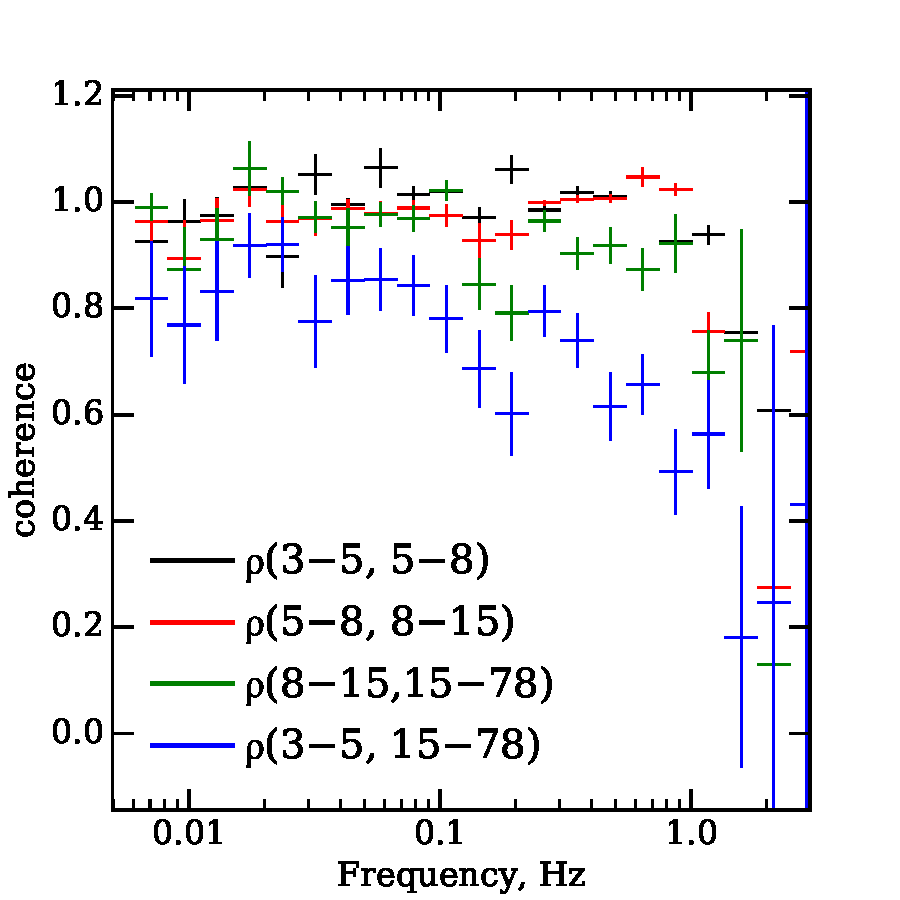
\includegraphics[width=\columnwidth]{coherence_4.pdf}
    \caption{Coherence between different energy bands:  red crosses between 3--5 and 5--8 keV,
     green crosses between 5--8 and 8--15 keV, blue crosses between 8--15 and 15--78 keV, black crosses between 3--5 and 15--78 keV.}
    \label{fig:coherence}
\end{figure}

The coherence between hard and soft energy bands at frequencies up to $\sim3$~Hz is presented in Fig.~\ref{fig:coherence}. 
We found that coherence in the adjacent energy bands is close to unity, with mean values in 0.01--1~Hz frequency band being $1.0\pm0.05$, however for the 3--5 and 15--78~keV energy bands the coherence is significantly lower, see Fig.~\ref{fig:coherence}. 
It is on the nearly constant level of $\approx0.85$ in the $5\times10^{-3}$--0.1~Hz frequency band and drops down above this frequency.
%Since the loss of the coherence is also observed above 0.3--1.0~Hz frequency for other energy bands, this effect may be connected not with the intrinsic properties of the source, but with the bead-time cross-talk effects which we did not specially consider, except for using light-curves from the different {\it NuSTAR} modules for cross-products.

\subsection{Phase lags}
        From the definition of the coherence (see eq.~\ref{eq:nowak_coh}) it follows that signals have roughly constant phase shifts between their Fourier functions in each frequency bin where they are coherent. 
Following \citet{1997ApJ...474L..43V} we estimated phase lag as an angle of mean product of the light curves Fourier harmonics from one energy bands to the conjugated Fourier harmonics of the second energy band. 
\begin{equation}
        \delta \phi(f) = \arctan{\left(\frac{Im(<F_{\rm s}^{*}(f) F_{\rm h}^{*}(f)>)}{Re(<F_{\rm s}^{*}(f) F_{\rm h}^{*}(f)>)}\right)}
\end{equation}
For the error estimation we used \citet{2014A&ARv..22...72U} approach, therefore $\Delta\delta\phi = \arctan{(\Delta\gamma^2/\gamma^2)}$, where $\gamma^2$ - estimation of the coherence, and $\Delta\gamma^2$ is coherence error estimation.
It should be noted that this estimation of the error is build on the assumption that each product $<F_{\rm h}^{*}(f) F_{\rm s}^{*}(f)>$ can be represented as a sum of randomly (for uncoherent signals) and particularly oriented (for coherent signals) vectors with constant length on complex plane, while it can be shown that, at least for uncoherent signals, that the length of this vectors is also random variable with Laplace distribution \citep{2017arXiv170909666H}.

We computed the phase lag spectrum with two approaches - with and without QPO centroid frequency tracing (see right and left panels of Fig.\ref{fig:phase_lag} correspondingly).
It appears that in the 0.1--3~Hz frequency band positive (hard) lag is present, on the frequencies below 0.1~Hz there are indication on the negative (soft) lag.
Observed phase lag corresponds to the delay times between soft and hard photons $\sim0.1$~s for frequencies above 0.1 Hz and $-0.1$..$-1$~s for frequencies below 0.1 Hz.
%The phase lag in the frequency range 0.1--3~Hz can be described with the shifted power law $\propto(f - f_0)^{0.3}$. 

\citet{2017ApJ...845..143Z} shown that the phase lag at the QPO frequency and its second harmonic in GX~339-4 BHC evolves with this frequency. 
It is also was shown by different authors \citep[see, e.g.,][]{2013ApJ...778..136P, 2017ApJ...845..143Z} that some distinct features are usually presented in phase lag spectra on the QPO and its harmonics frequencies, however, our signal to noise ratio appears to be insufficient to determine the presence of such features.
\citep{2017MNRAS.464.2643V} shown that the sign of the phase lag on the type-C QPO centroid frequency depends on a system inclination, however this difference is explicit only when QPO centroid frequency is above $\sim3$~Hz.


\begin{figure*}
        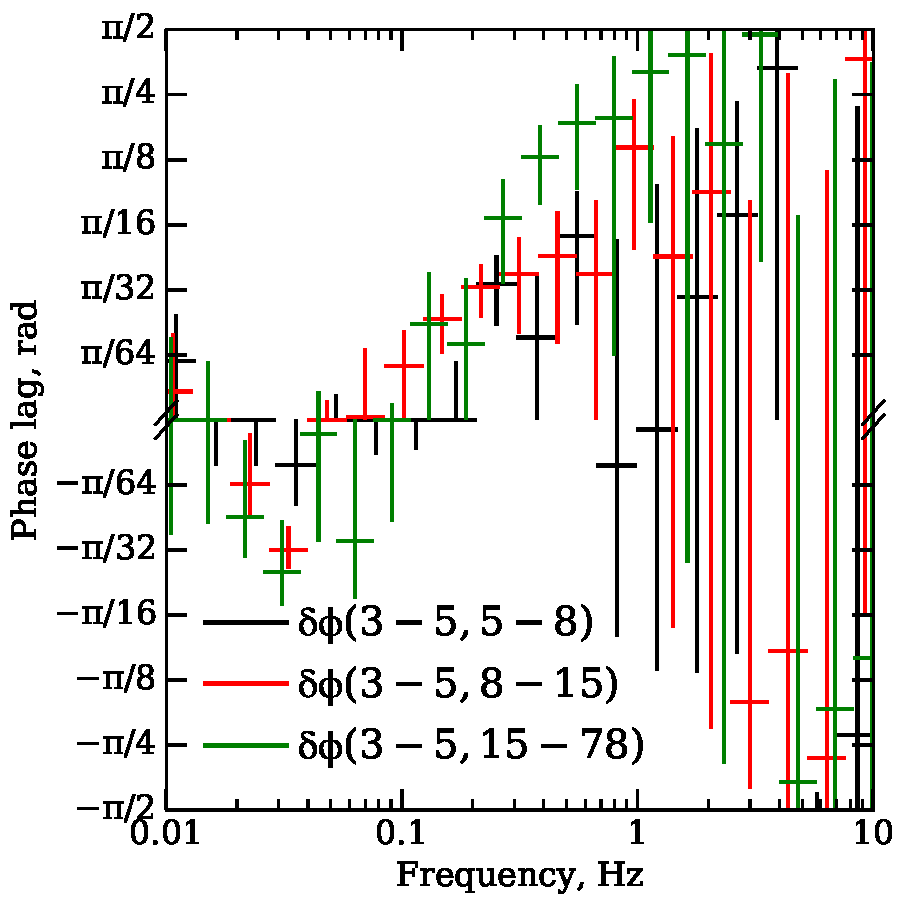
\includegraphics[width=0.99\columnwidth]{phase_lag_untracked.pdf}
        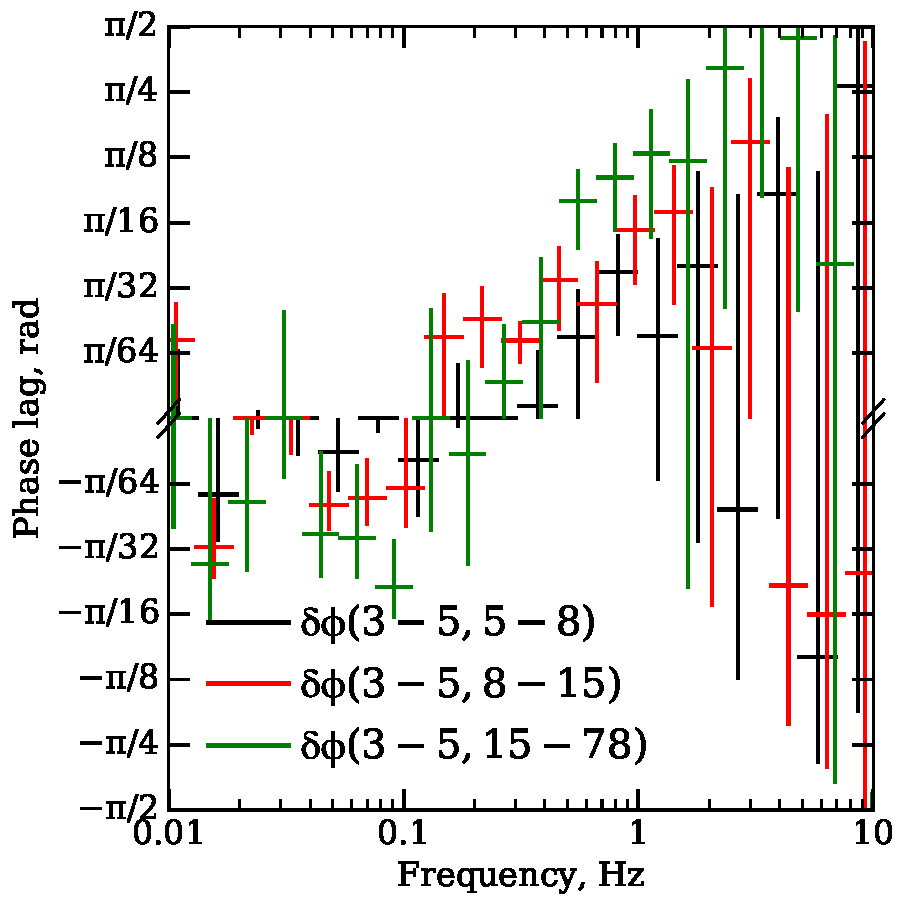
\includegraphics[width=0.99\columnwidth]{phase_lag_new.pdf}
        \caption{Phase lag between the soft (3--5~keV) and hard (5--8; 8--15; 15--78~keV) energy bands in \grs. 
        On the left panel - phase lag spectrum obtained from {\it NuSTAR} observations by stacking all data, on the right panel same spectrum with tracked frequency (frequency for each separate light-curve segment was scaled such a way to conserve QPO centroid at 0.3~Hz).}
        \label{fig:phase_lag}
\end{figure*}

\subsection{\swiftx\, observations}
We performed search for LF QPOs in first dozen of \swiftx observations of the \grs. 
QPO is clearly detected in observations 3 to 9, with frequency varying from 0.4 Hz (during simultaneous observation with \nustar, see Fig.~\ref{fig:nust_lc}) up to 5 Hz (see Tab.~\ref{tab:xrtqpo}). 
Due to typically short exposures of \swiftx\, snapshots (about 1 ks) it is hard to classify QPOs as belonging to type C or B, because low-frequency part of power spectra lacks statistics, yet, except for the first detection (observation 03) power spectra were red-noise like, without strong low-frequency components. 
We calculated $rms$ for each detected QPO - most of them is higher than 10\%, which is not typical for type C QPO \citep{casella05}.

\begin{table}
\noindent
\centering
\caption{QPOs detected in \swiftx\, observations}
\label{tab:xrtqpo}
\centering
\begin{tabular}{|c|c|c|c|}
\hline\hline
Segment & $f_{QPO}$, Hz & $rms$, \% & Type\\
\hline
03  &  0.4  &  14\% & C\\
04  &  2.2 &  11\% & B\\
05  &  1.7  & 13\% & B \\ 
06  &  5.0 &   6\% & B\\
07  &  2.5 &  10\% &  B\\ 
08  &  5.1 &   7\% & B\\
09  &  2.2 &  11\% &  B\\
\hline
\end{tabular}
\end{table}

\section{Discussion and conclusions}
We had studied the spectro-timing evolution of \grs\, during its hard-intermediate state.  
We found a prominent type-C LF QPO in its power spectrum, its frequency show clear correlation with parameters of continuum emission. 
As the QPO frequency increases from 0.3 to 0.7 Hz spectrum became softer: the power law index grows from 1.46 to 1.53 and cut-off energy decreases from 30 to 26 keV. 
Overall flux increases, too. 
Such behaviour was first observed in a number of systems by \citet{dimatteo99} and now it is studied in greater details in many systems \citep[see e.g.][ and many more]{vignarca03,stiele13,seifina14,fuerst16_gx339}. 
Although the quality of a data prevented us from measuring a movement of the inner disk boundary, from the total broadband spectrum we found that an accretion disk is truncated at radius smaller than 9 $GM/c^{2}$ (90\% confidence limit) which is in agreement with an estimates by \citet{miller15_nust}. 
We used this combination of inner radius and QPO together with Lense-Thirring precession model of QPO origin \citep{ingram09} in order to assess black hole mass. 
Following \citet{ingram14} we calculated nodal frequencies (which is though to correspond to QPO fundamental frequency) versus inner radius for two values of the black hole mass (10$M_{\odot}$ and 30$M_{\odot}$) and two values of spin - $a=0.1$ and $a=0.998$ (maximally rotating). 
As it can be seen from Fig.~\ref{fig:qpoconstr} observations are incompatible with black hole mass 10$M_{\odot}$ and barely agrees with slowly rotating massive black hole. 
This results, along with measurements by \cite{fuerst16_gx339}, indicate that there are some tensions between predictions of RPM and truncation radii inferred from spectral fitting.

\begin{figure}
        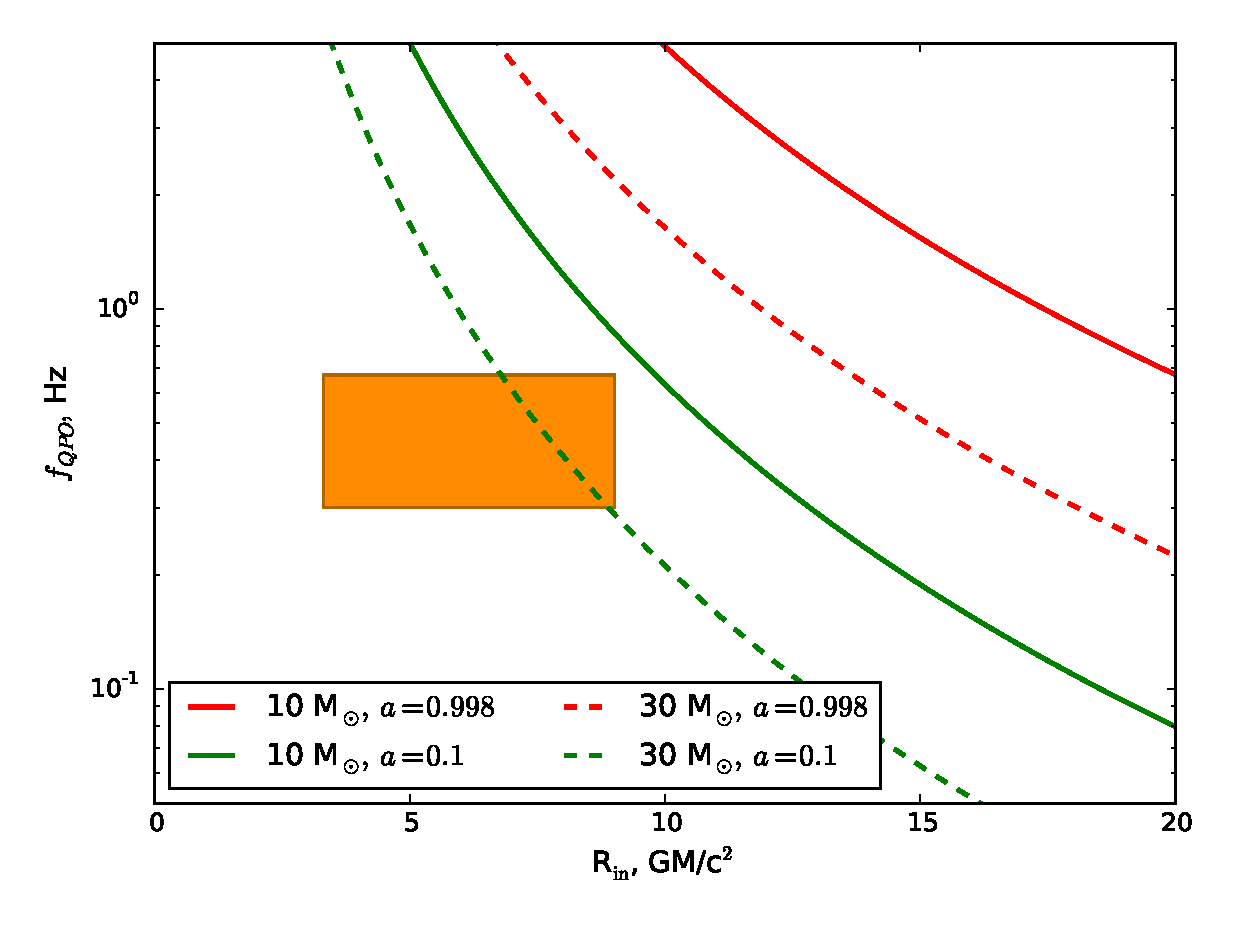
\includegraphics[width=\columnwidth]{qpoconstr_v03.eps}
        \caption{Expected QPO frequency for a black hole of a given mass and spin versus inner disk radius from \protect\cite{ingram14}. Orange square represent region containing observed QPOs.}
        \label{fig:qpoconstr}
\end{figure}

We carried out extensive study of timing properties of the \grs. 
Along with the broadband noise and fundamental QPO, second harmonic of QPO is clearly seen. 
During several intervals from first half of the observation subharmonic is also observed. 
%Break frequency of broadband noise is correlated with QPO frequency following the WK relation \citep{wijnands99}. 
In all 13 intervals second QPO harmonic is more prominent in soft band (3--5 keV), with ratio of its amplitude to that of fundamental QPO being $0.565\pm0.02$ in 3--5 keV band versus $0.275\pm0.02$ in 15--78 keV.  
We also measured velocity of the QPO drift and found it to be $\approx6.0\times10^{-6}$~Hz~s$^{-1}$. 
We searched for similar QPO in \swiftx\, observations of \grs\ performed after \nustar\, exposure and found that all other detected QPOs are probably of type B, thus indicating that the type-C QPO reach saturation on frequencies below few Hz. 
Coherence measured between adjacent energy ranges in 0.01-1 Hz was found to be nearly unity, while for distant energy bands coherence turned out to be lower. 
Phase lag found to be of order of $+0.1$~s (hard) in the 0.1--3~Hz frequency range and $-1$..$-0.1$~s (soft) below 0.1~Hz.


\section*{Acknowledgments}
The work was supported by the Russian Science Foundation (grant no. 14-12-01287). Authors are grateful for T.Dauser and J.Gracia for their help with {\em relxill} model. 
This research has made use of data obtained through the High Energy Astrophysics Science Archive Research Center Online Service, provided by the NASA/Goddard Space Flight Center.


%--------------------------------------------------------------------------------
\bibliographystyle{astron}
\bibliography{author_en.bib,coherence.bib}
\bsp	
\label{lastpage}
\end{document}
